\documentclass[11pt]{article}
%Gummi|065|=)
\title{\textbf{Meccano heptagons}}
\author{https://github.com/heptagons/meccano/hepta}
\date{}

\usepackage{amsmath}
\usepackage[pdftex]{graphicx}
\usepackage{listings}
\usepackage{xcolor}
\definecolor{gray}{RGB}{245,245,245}
\usepackage{hyperref}

\lstset{
	backgroundcolor=\color{gray},
	frame=single,
	language=c,
	numbers=left,
	stepnumber=1
}

\usepackage[margin=0.75in]{geometry}

% inkscape fig.svg --export-pdf=fig.pdf (prior version 1.0)

\usepackage{graphicx}
\begin{document}

\maketitle

\section{Meccano heptagons}

\begin{figure}[htp]
\centering
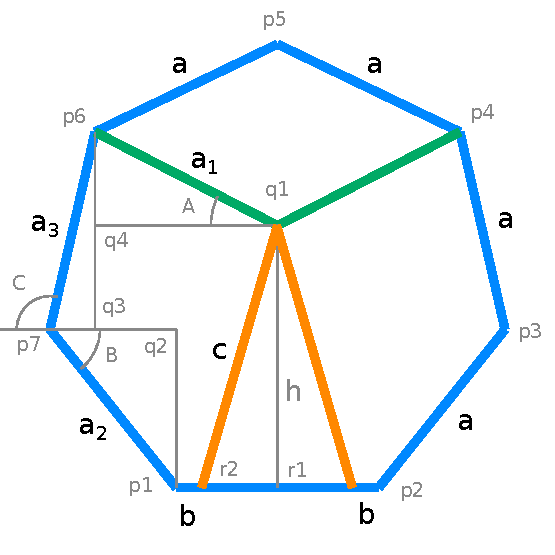
\includegraphics[scale=1]{figs/heptagon_plan.pdf}
\caption{A meccano regular heptagon layout. First we define two integers $a$ and $b$ where $a > 2b$. We look for a third integer $c$ to make the heptagon.}
\label{heptagonplan}
\end{figure}

Consider the regular heptagon in figure \ref{heptagonplan}.
By inspection we identify three angles $A$, $B$ and $C$:

\begin{align*}
A &= \frac{\pi}{7} \\
B &= \frac{2\pi}{7} \\
C &= \frac{4\pi}{7} \\
\end{align*}

Then we find the sines of the angles, noticing that the regular heptagon side is $a = a_1 = a_2 = a_3$:

\begin{align*}
sinA &= \frac{\overline{p_6 q_4}}{a_1} \\
sinB &= \frac{\overline{p_1 q_2}}{a_2} \\
sinC &= \frac{\overline{p_6 q_3}}{a_3} \\
\end{align*}

From the figure the height $h$ corresponds to:

\begin{align*}
h &= \overline{p_1 q_2} + \overline{p_6 q_3} - \overline{p_6 q_4} \\
  &= a_2sinB + a_3sinC - a_1sinA \\
  &= a(-sinA + sinB + sinC)\\
\end{align*}

According to \emph{heptagonal triangles}\footnote{https://en.wikipedia.org/wiki/Heptagonal\_triangle}

\begin{align*}
sinA - sinB - sinC &= -\frac{\sqrt{7}}{2} \\
       \frac{h}{a} &= \frac{\sqrt{7}}{2} \\
                 h &= \frac{\sqrt{7}a}{2}
\end{align*}


Finally we get the $c$ length as a function of lengths $a$ and $b$:

\begin{align*}
c^2 &= \overline{r_1 r_2}^2 + h^2 \\
    &= \frac{(a - b)^2}{4} + \frac{7a^2}{4} \\
    &= \frac{8a^2 - 2ab + b^2}{4}
\end{align*}

\subsection{Heptagons search}

A valid meccano heptagon needs to have the three lenghts $a$, $b$ and $c$ as integers. With a software routine we look for c to be integer by incrementing the values of $a > b$.

\subsubsection{Code}

Following javascript code running inside a web page is used to find several heptagons:

\begin{lstlisting}
<script type="text/javascript">
const gcd = (a, b)=> { return !b ? a : gcd(b, a % b) } 

let i = 1
for (let a=2; a <= 100; a++) {
  for (let e=1; e < a; e++) {
    const c = Math.sqrt(7*a*a + e*e)/2;
    if ((c - parseInt(c)) == 0) {
      if (gcd(c, gcd(a, e)) == 1) {
        console.log(`N=${i}: a=${a} b=${(a-e)/2} c=${c}`);
        i++;
      }
    }
  }
}
</script>
\end{lstlisting}

\subsubsection{Results}

Browser console first heptagons with $a < 100$:

\begin{lstlisting}
N= 1: a= 3 b= 1 c=  4
N= 2: a= 8 b= 1 c= 11
N= 3: a=33 b= 2 c= 46
N= 4: a=40 b=17 c= 53
N= 5: a=55 b=14 c= 74
N= 6: a=65 b=31 c= 86
N= 7: a=85 b=14 c=116
N= 8: a=91 b= 2 c=128
N= 9: a=95 b= 1 c=134
N=10: a=96 b=47 c=127
\end{lstlisting}

\subsubsection{Smallest examples}

\begin{figure}[htp]
\centering
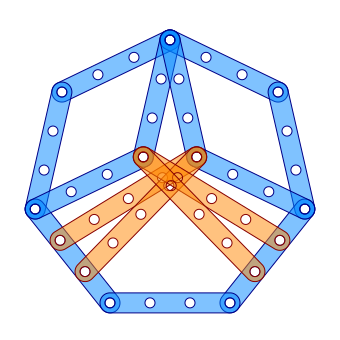
\includegraphics[scale=1]{figs/heptagon-3}
\caption{The first meccano heptagon with values $a=3$, $b=1$ and $c=4$.}
\label{heptagon-3}
\end{figure}

\begin{figure}[htp]
\centering
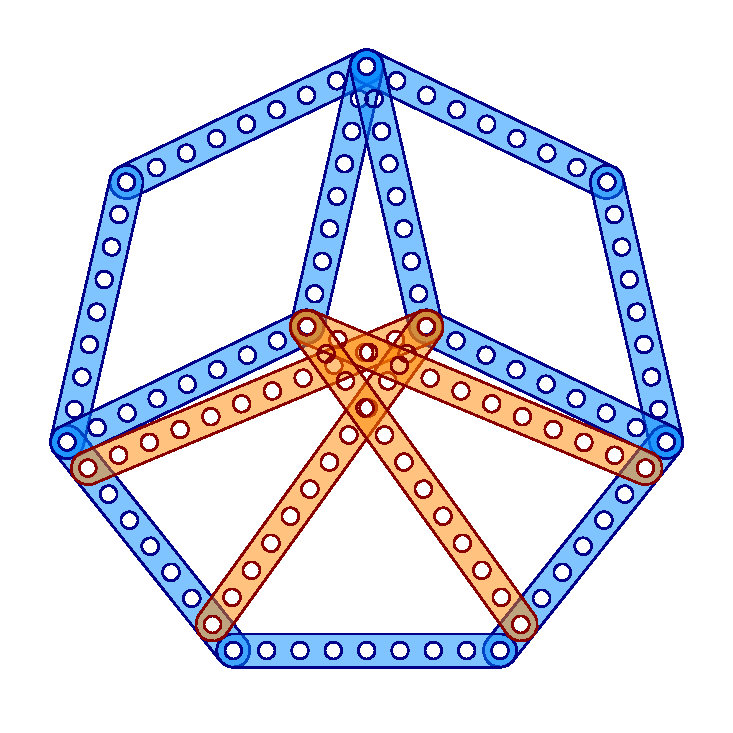
\includegraphics[scale=1]{figs/heptagon-8}
\caption{The second meccano heptagon with values $a=8$, $b=1$ and $c=11$.}
\label{heptagon-8}
\end{figure}

Figures \ref{heptagon-3} and \ref{heptagon-8} show the first two heptagons.






\end{document}

